\documentclass[landscape]{slides}
\usepackage[landscape, margin=2cm]{geometry}
\usepackage{color}
\usepackage{bm}
\usepackage{graphicx}
\usepackage{hyperref}
\graphicspath{ {./img/} {./charts/} }



\title{Show and Tell: Skill Acquisition}
\author{Adam Johnson - me@adamj.eu}
\date{28th August 2013}

\begin{document}

\maketitle


\begin{slide}

    \textcolor{blue}{\Large{Skill Acquisition}}

    \begin{itemize}
        \item I have been re-learning a skill recently
        \item I tracked myself doing it
        \item This is the story...
    \end{itemize}

\end{slide}



\begin{slide}

    \textcolor{blue}{\Large{The Skill}}

    \begin{itemize}
        \item A puzzle for you...
    \end{itemize}

    % - something you did today
    % - you've been paid to do it
    % - you've probably never practiced it in your life

    % no, it's not making tea...

\end{slide}


\begin{slide}

    \textcolor{blue}{\Large{Typing!}}

    \centering

    
\includegraphics[height=10cm]{baby-nerd}

    (not me)

\end{slide}


\begin{slide}

    \textcolor{blue}{\Large{Motivation}}

    \begin{itemize}
        \item I'm a programmer - I have a lot of typing to do!
        \item Fear of RSI - both Mum and colleague have both been crippled by it
        % \item Always \emph{intended} to learn to touchtyping
        \item Stat: ``In the USA, carpal tunnel syndrome results in an average of \$30,000 in lifetime costs'' (Wikipedia)
    \end{itemize}

\end{slide}


\begin{slide}

    \textcolor{blue}{\Large{To business!}}

    \begin{itemize}
        \item Just need to grab some typing programs
        \item Get down to learning QWERTY the \emph{right} way!!
    \end{itemize}

\end{slide}


\begin{slide}

    \centering

    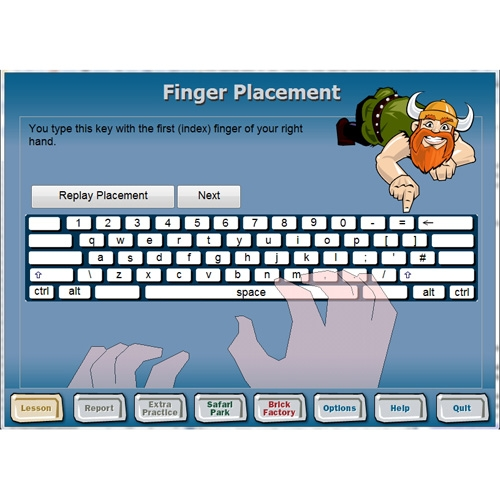
\includegraphics[height=19cm]{ten-thumbs}

\end{slide}


\begin{slide}

    \textcolor{blue}{\Large{Oh no....}}

\end{slide}

\begin{slide}
    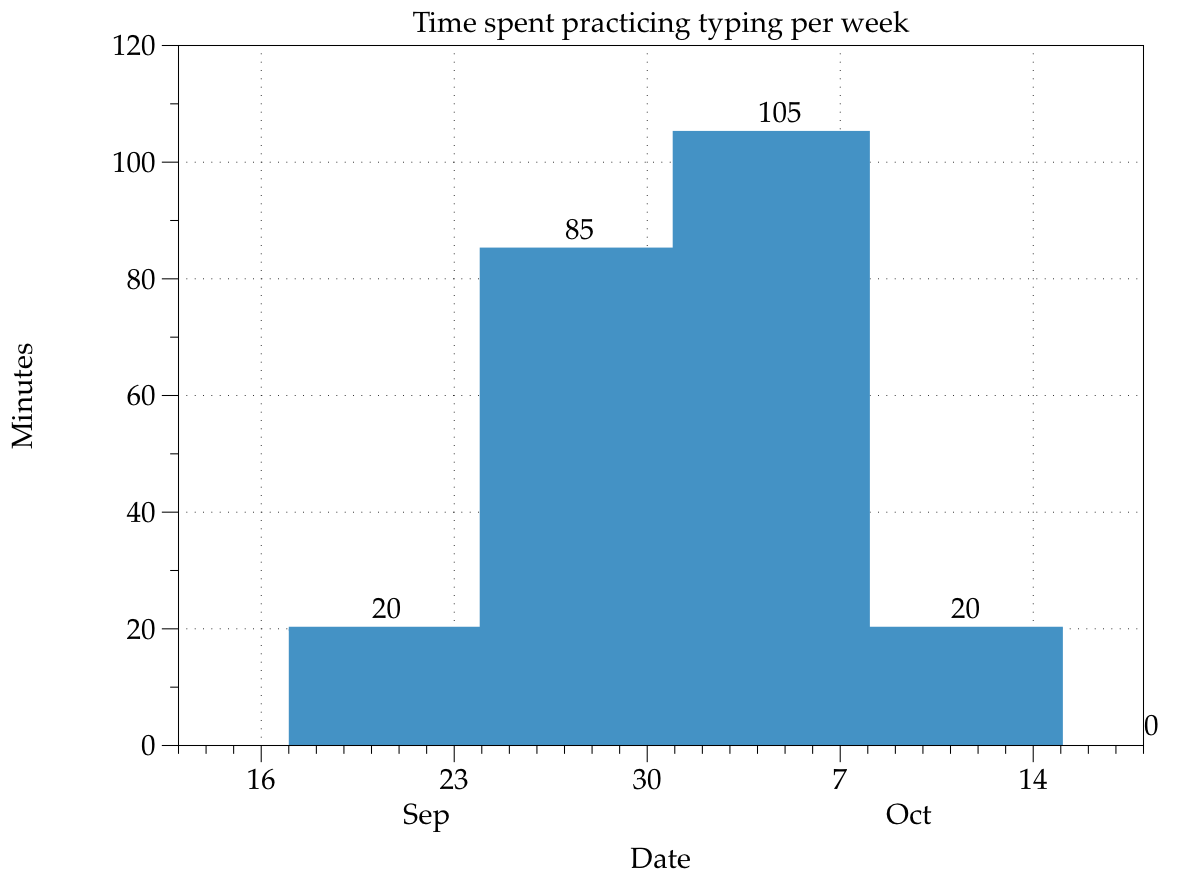
\includegraphics[width=\textwidth]{first-practice}
\end{slide}

\begin{slide}
    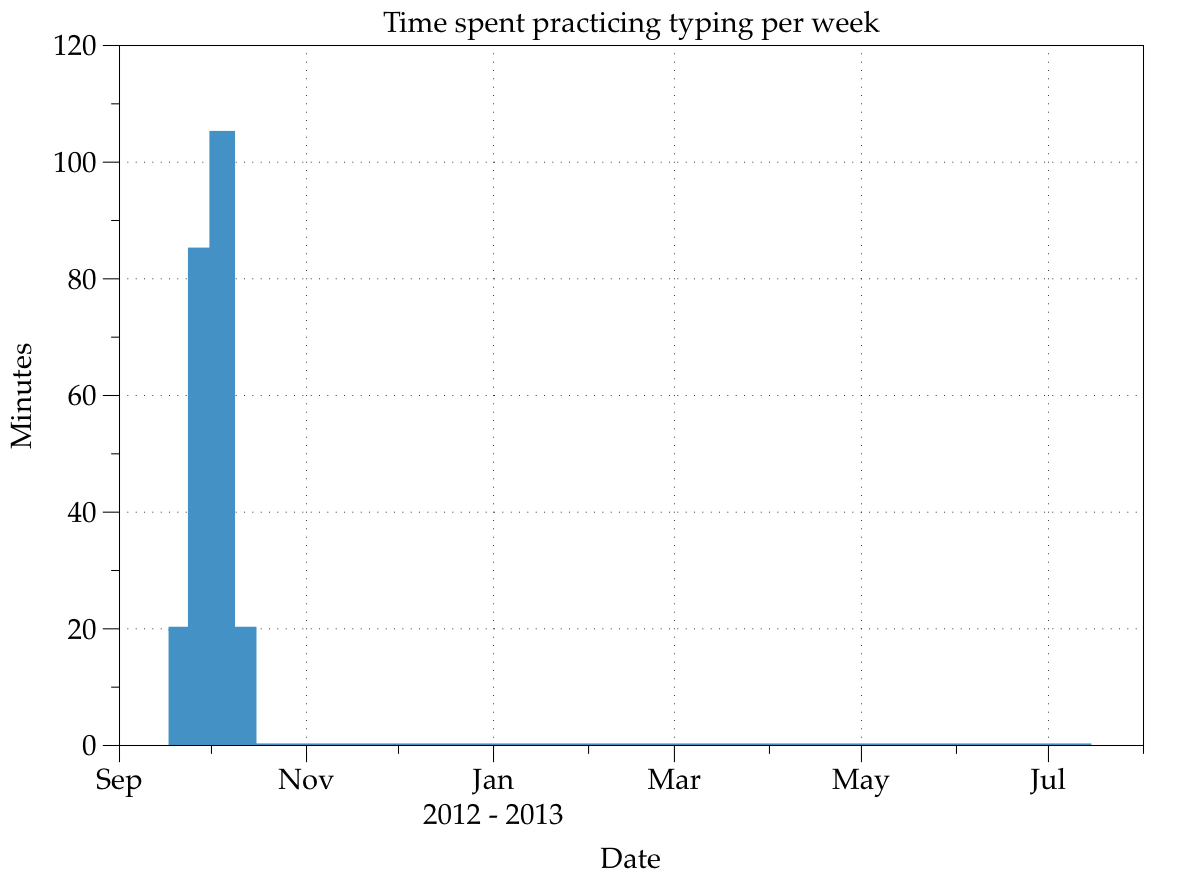
\includegraphics[width=\textwidth]{first-practice-long-tail}
\end{slide}


\begin{slide}

    \textcolor{blue}{\Large{Under-motivation}}

    \begin{itemize}
        \item Didn't know how long it would take
        \item Relative size of advantage
        \item Hard practicing QWERTY \emph{the right way} at night, then going back to old habits during the day
    \end{itemize}

\end{slide}


\begin{slide}

    \textcolor{blue}{\Large{So what changed?}}

\end{slide}


\begin{slide}

    \textcolor{blue}{\Large{The First 20 Hours}}

    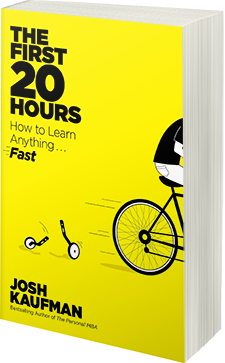
\includegraphics[height=10cm]{first20hours-cover}

    \begin{itemize}
        \item Josh Kaufman, 2013
        \item \url{http://first20hours.com/}
    \end{itemize}

\end{slide}


\begin{slide}

    \textcolor{blue}{\Large{The First 20 Hours : Rapid Summary}}

    \begin{itemize}
        \item Nearly any skill can be learnt to a useful degree in 20 hours
        \item A couple chapters of general how-to, then one chapter on each skill he learnt with his method
        \item One of these was on touchtyping... in `Colemak'
    \end{itemize}

\end{slide}


\begin{slide}

    \textcolor{blue}{\Large{QWERTY}}

    \centering
    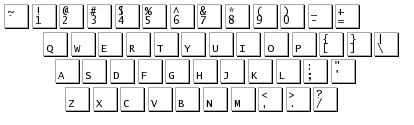
\includegraphics[width=20cm]{qwerty}

    \begin{itemize}
        \item ``Slowly took over the world'', since 1872. Main design constraint: to stop typewriter key bars jamming.
    \end{itemize}

\end{slide}


\begin{slide}

    \textcolor{blue}{\Large{DVORAK}}

    \centering
    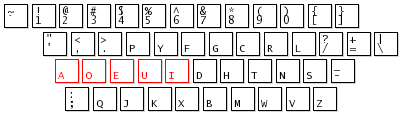
\includegraphics[width=20cm]{dvorak}

    \begin{itemize}
        \item 1932 attempt at optimisation. Relatively hard to learn.
    \end{itemize}

\end{slide}


\begin{slide}

    \textcolor{blue}{\Large{Colemak}}

    \centering
    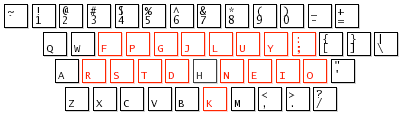
\includegraphics[width=20cm]{colemak-annot}

    \begin{itemize}
        \item Designed by a programmer with mathematical models. Split between ease of transition (Q,W,Z,X,C,V stay the same) and optimization.
    \end{itemize}

\end{slide}


\begin{slide}

    \centering

    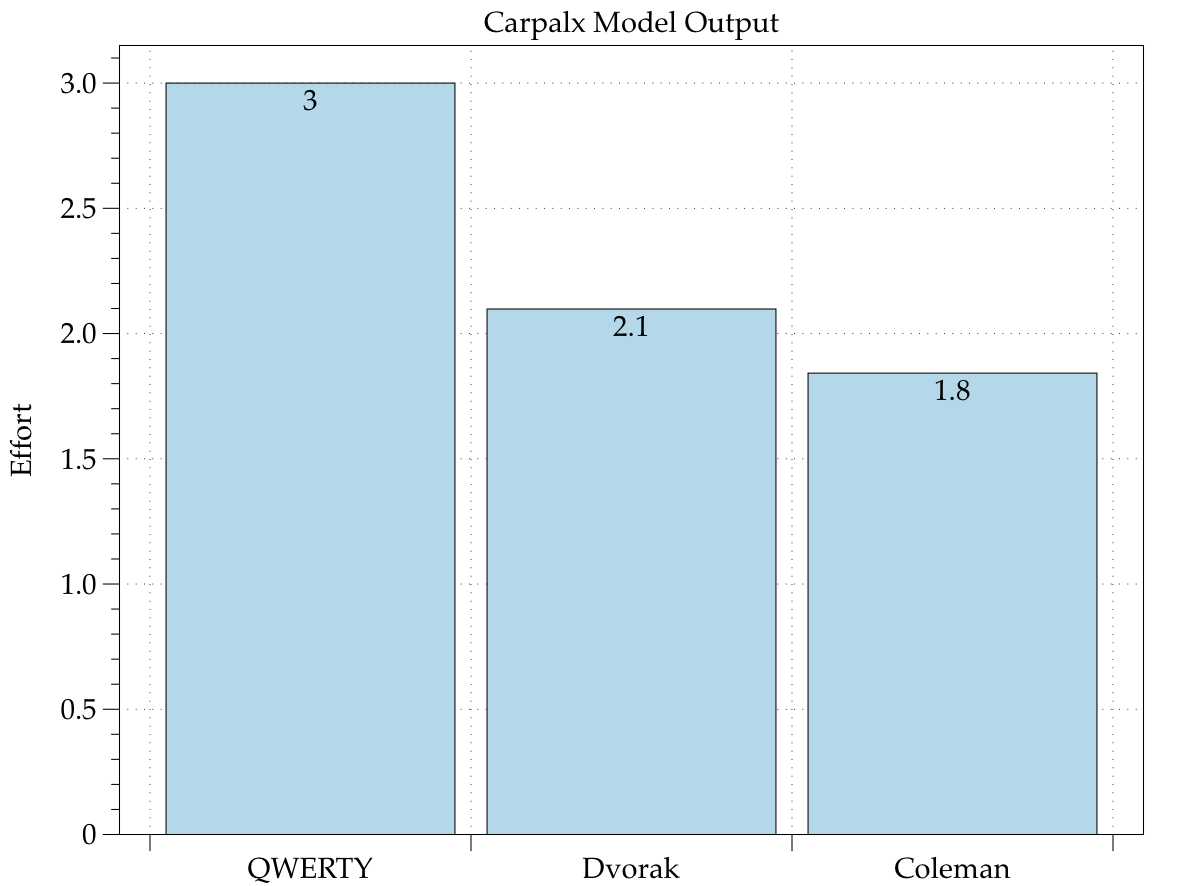
\includegraphics[width=0.85\textwidth]{keyboards}

    \begin{itemize}
        \item Source: \url{http://mkweb.bcgsc.ca/carpalx/?colemak}
    \end{itemize}

\end{slide}


\begin{slide}

    \textcolor{blue}{\Large{Method}}

    \begin{itemize}
        \item Swap keys on OS and keyboard
        \item Get some training programs
        \item Fire away
    \end{itemize}

\end{slide}


\begin{slide}

    \textcolor{blue}{\Large{Method}}

    \begin{itemize}
        \item Swap keys on OS and keyboard
        \item Get some training programs
        \item Try to practice in 20 minute + sessions, before bed.
    \end{itemize}

\end{slide}


\begin{slide}

    \textcolor{blue}{\Large{Programs}}

    \begin{itemize}
        \item A good mix of programs is useful
        \item Practice different subskills - hardest keys, whole prose, etc.
        \item Data export - not much of a feature here. Many record your WPM + accuracy, but hard to know
    \end{itemize}

\end{slide}


\begin{slide}

    \textcolor{blue}{\Large{Amphetype}}

    \centering

    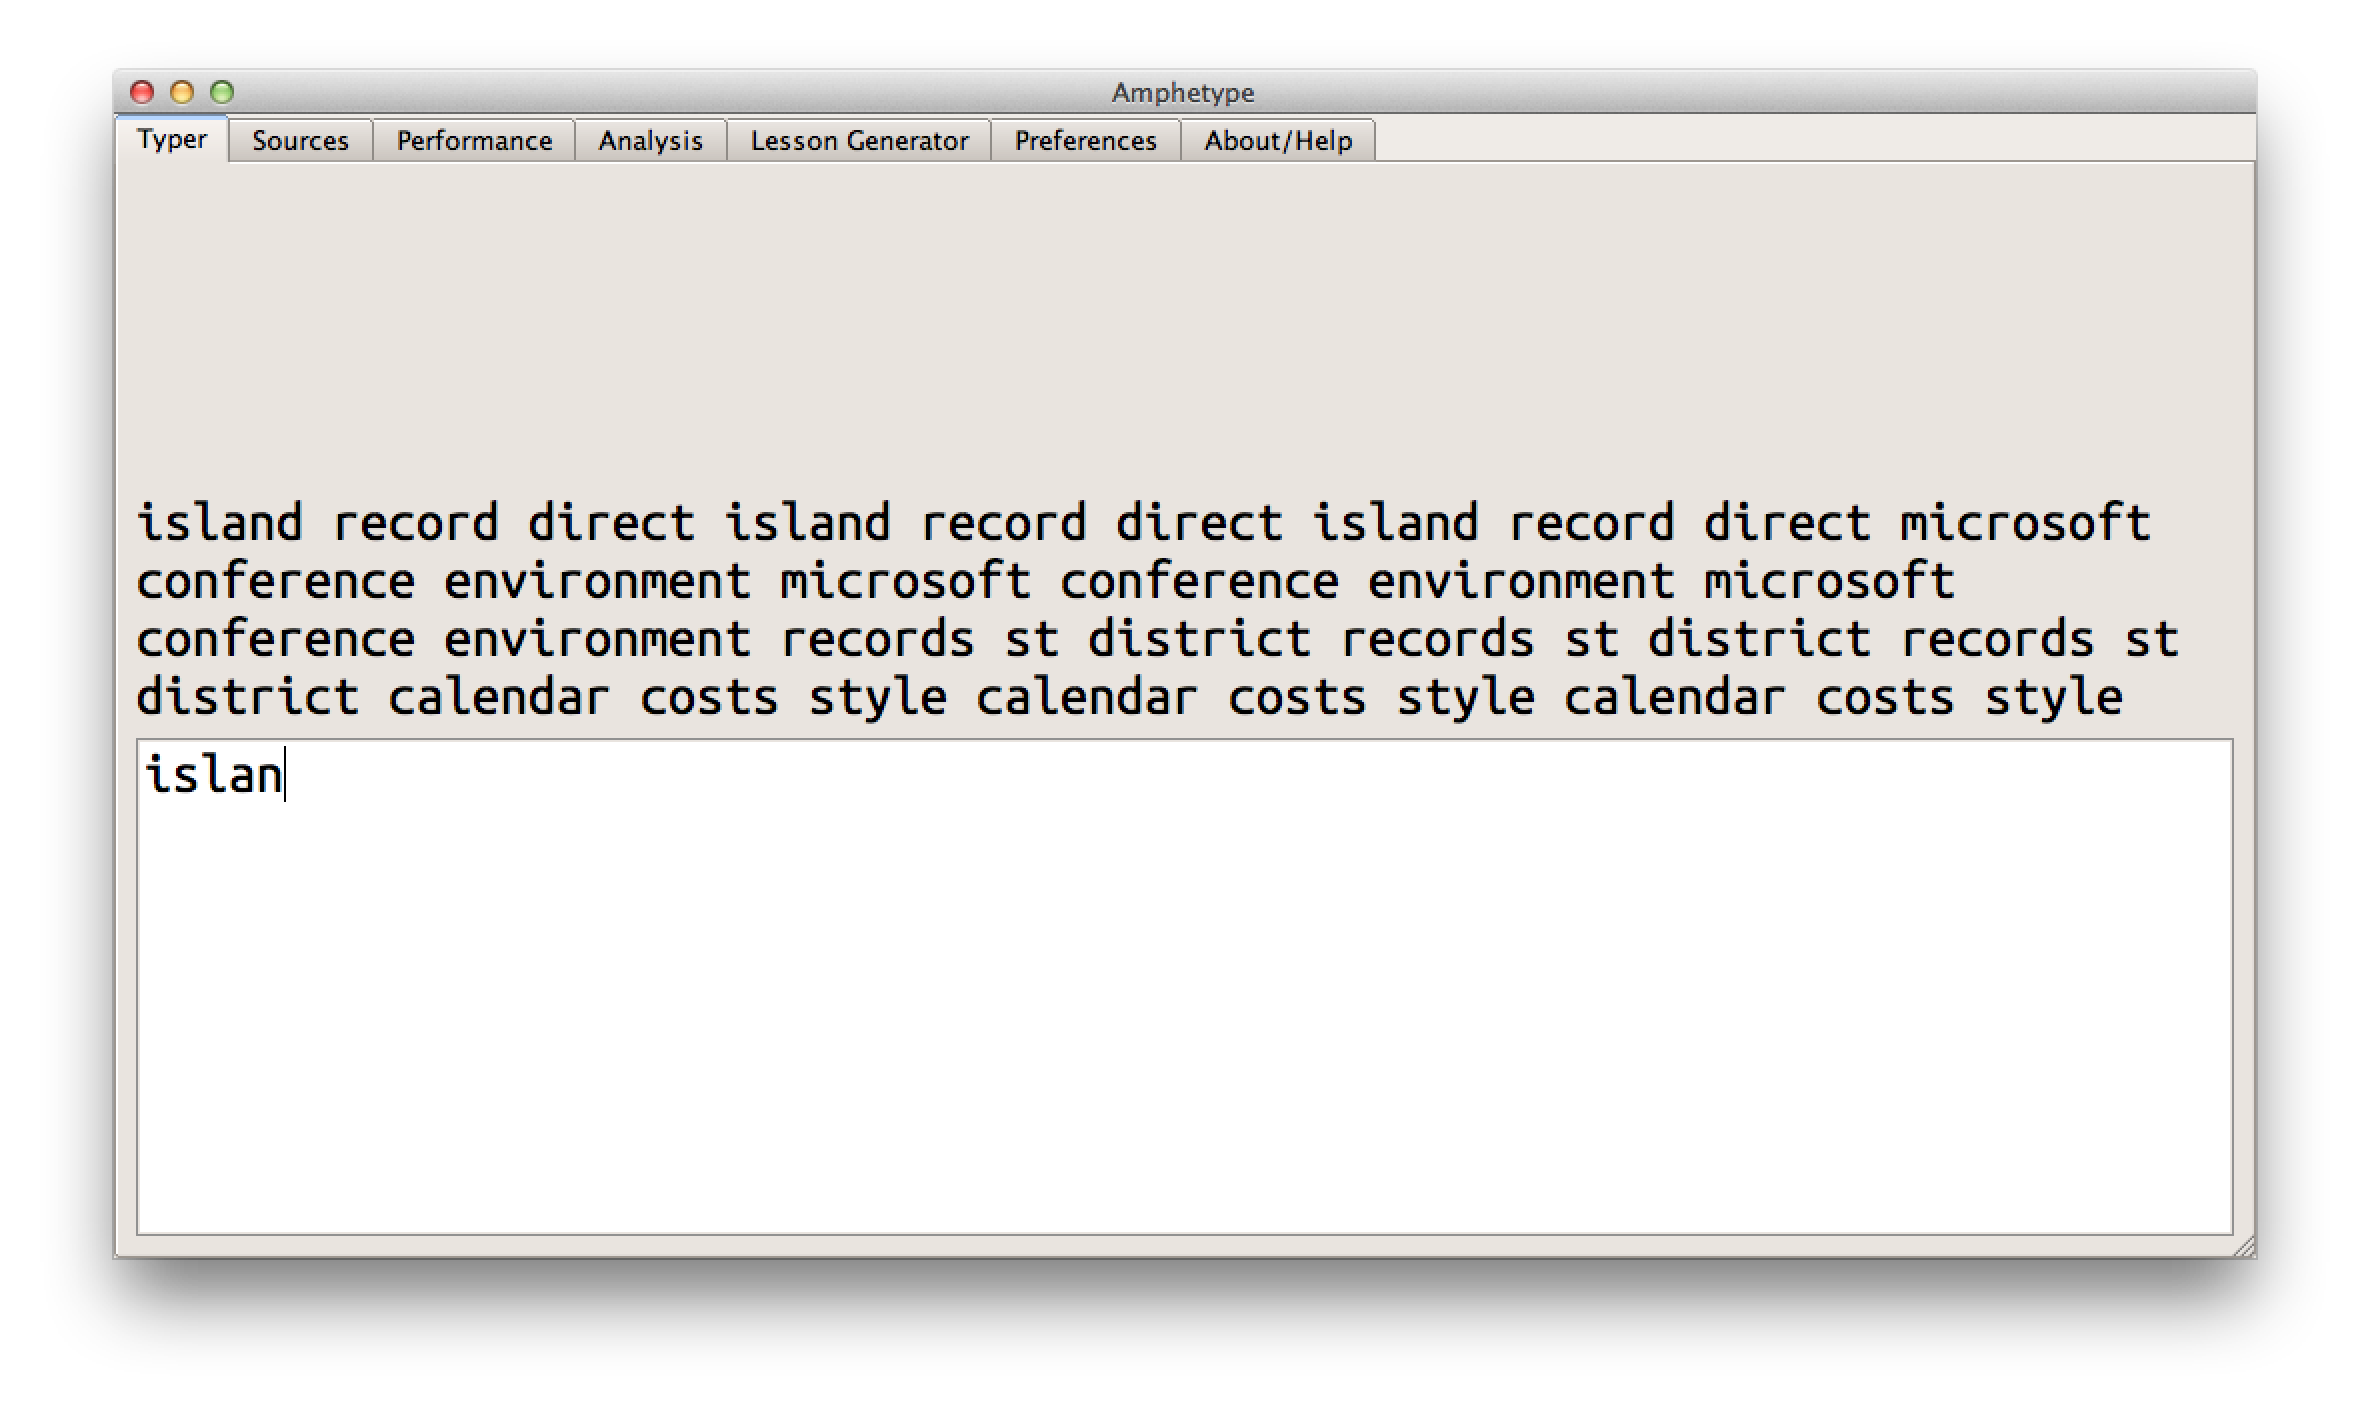
\includegraphics[width=0.8\textwidth]{amphetype-screenshot}

    \begin{itemize}
        \item Free \& open source - \url{https://code.google.com/p/amphetype/}
    \end{itemize}

\end{slide}


\begin{slide}

    \textcolor{blue}{\Large{Type-Fu}}

    \centering

    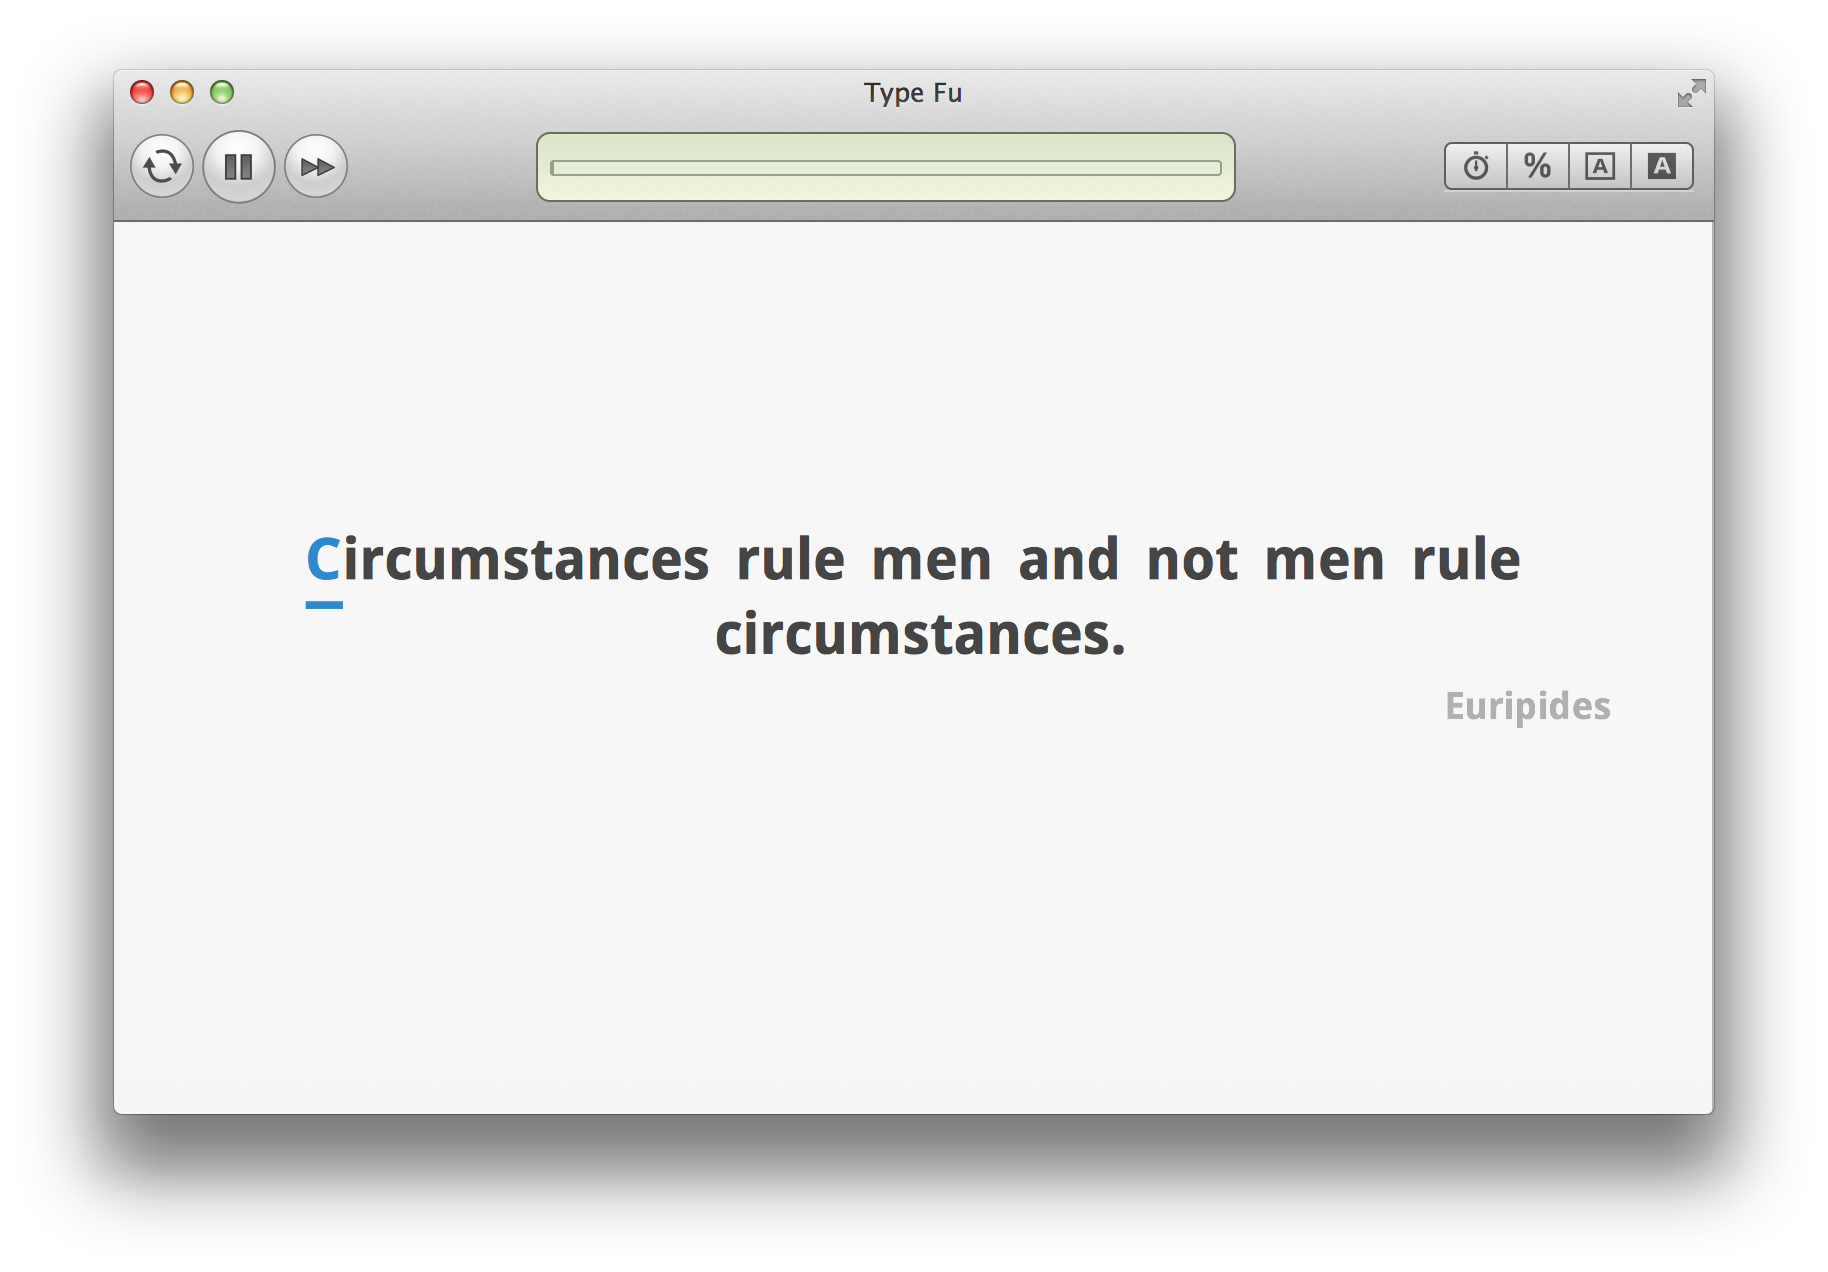
\includegraphics[width=0.8\textwidth]{type-fu-screenshot}

    \begin{itemize}
        \item £6.99 - \url{http://type-fu.com/}
    \end{itemize}

\end{slide}


\begin{slide}

    \textcolor{blue}{\Large{Typocalypse 3D}}

    \centering

    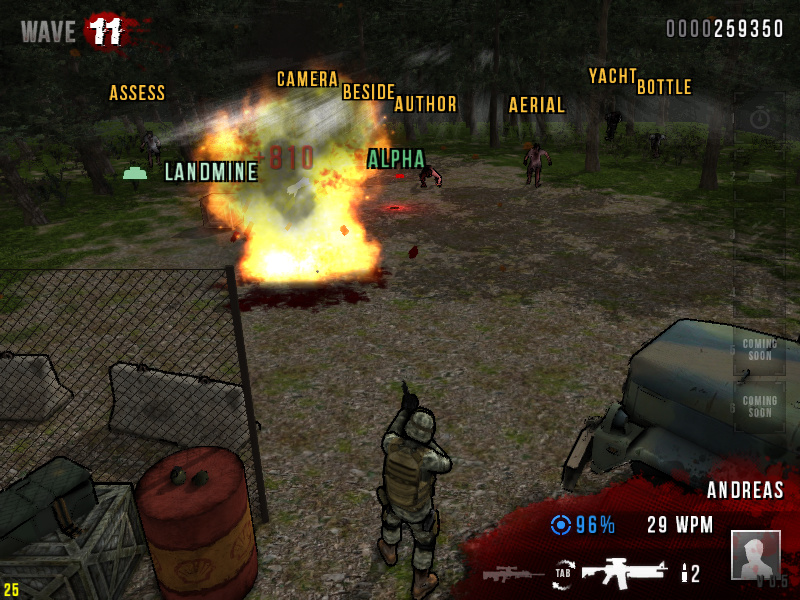
\includegraphics[width=0.75\textwidth]{typocalypse-3d}

    \begin{itemize}
        \item Free - \url{http://is.gd/typeocalypse}
    \end{itemize}

\end{slide}


\begin{slide}

    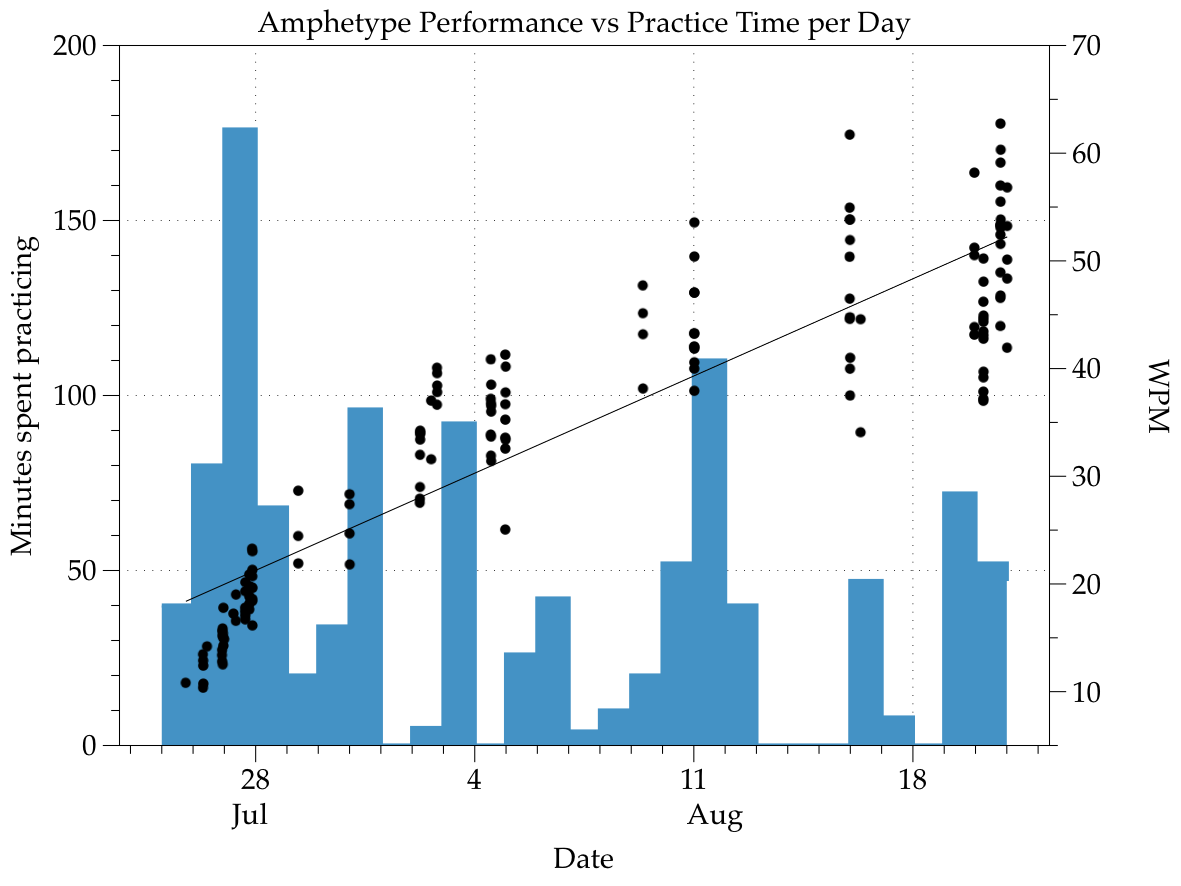
\includegraphics[width=\textwidth]{amphetype}

\end{slide}


\begin{slide}

    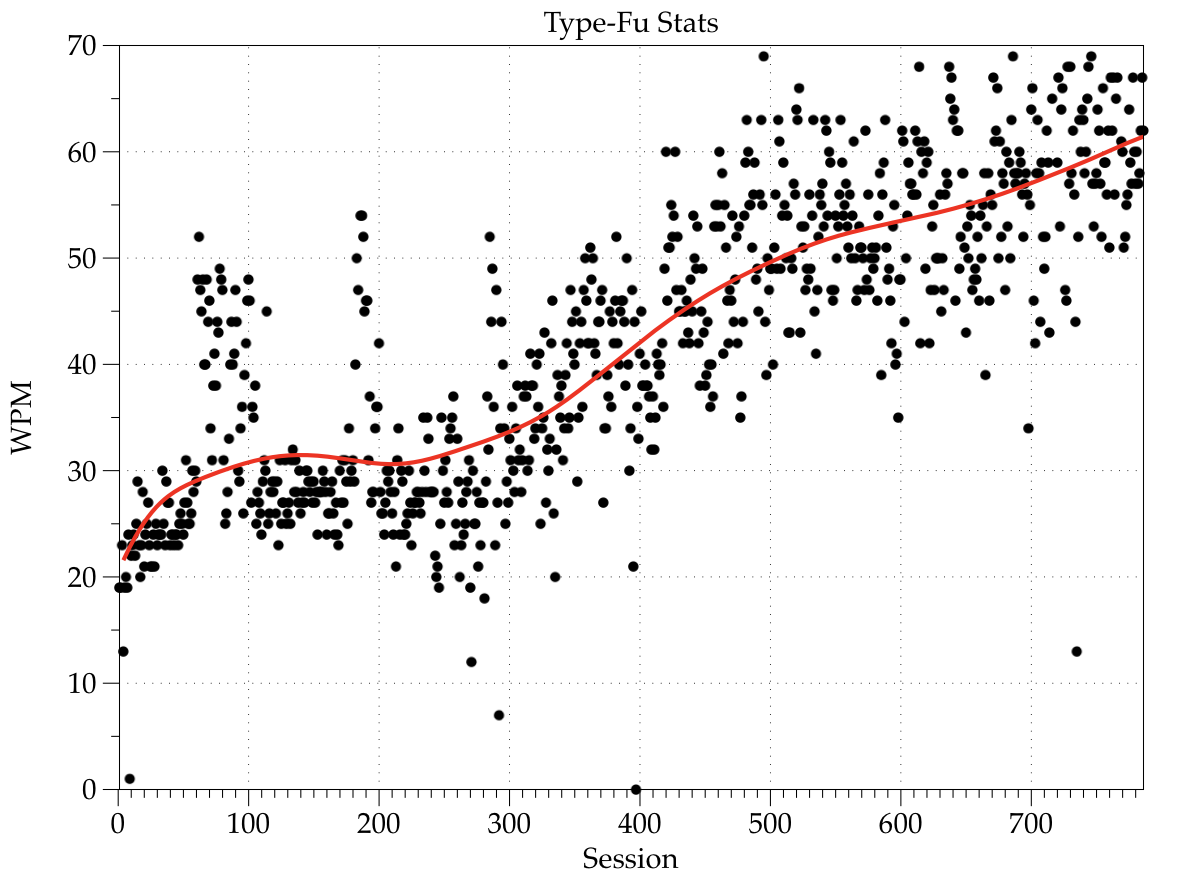
\includegraphics[width=\textwidth]{type-fu}

\end{slide}


\begin{slide}
    \textcolor{blue}{\Large{Thank you}}

    \begin{itemize}
        \item Slides on GitHub - \url{http://is.gd/adamIsDaBomb}
        \item Email me - \url{me@adamj.eu}
    \end{itemize}

\end{slide}


\end{document}
